\section*{Energy Calibration}

The first task is the energy calibration of the three detectors:
\begin{itemize}
\item Tagger
\item Scatterer
\item Detector
\end{itemize}
For the purpose of energy calibrating these detectors two different radioactive source were used:
\begin{enumerate}
\item $^{22}$Na: with two different photopeak at 511 keV and 1275 keV
\item $^{241}$Am: with a photopeak at 59.5 keV
\end{enumerate}

Calibrated spectra are showed in Fig. \ref{Fig: calibrated spectra}.
\begin{figure}[H]
\centering
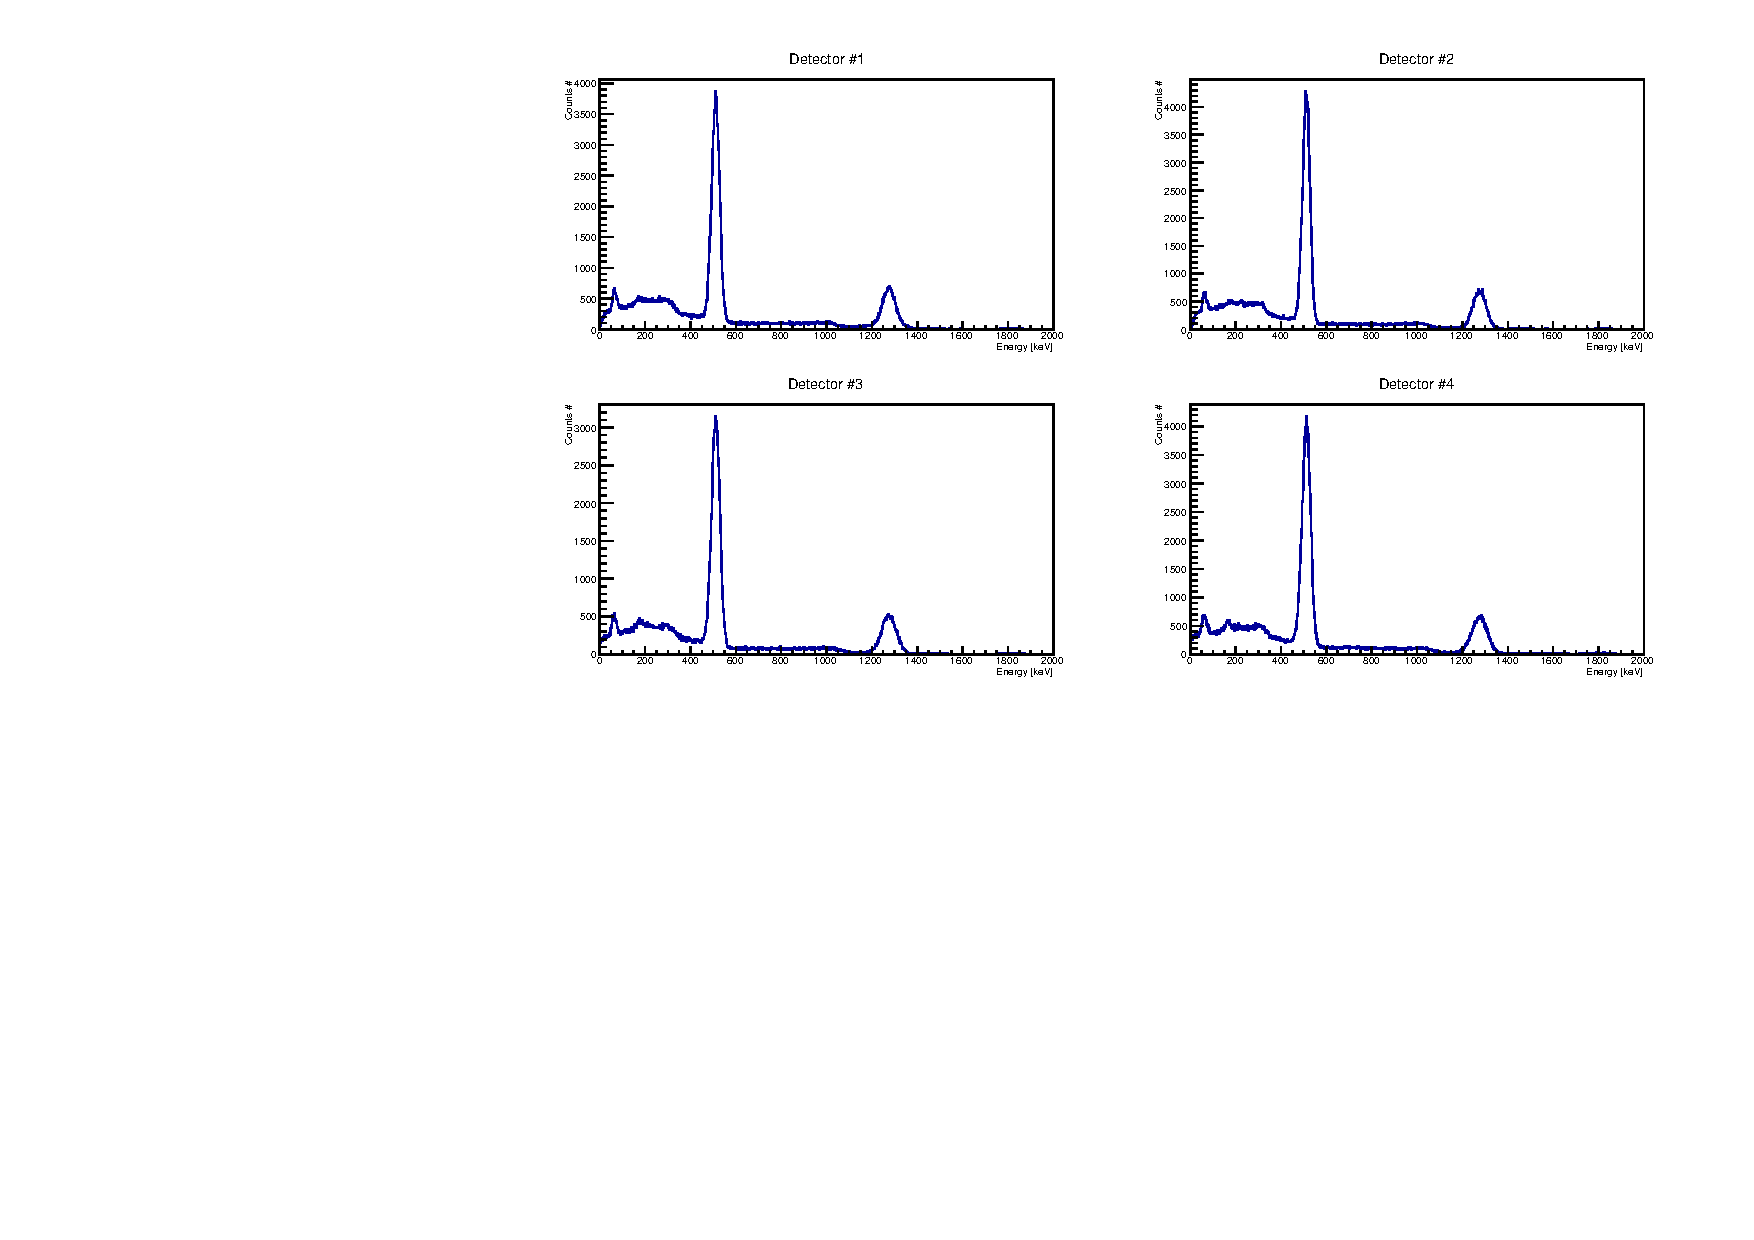
\includegraphics[width = \textwidth]{calibrated_spectra}
\caption{Calibrated $^{22}$Na energ spectrum.}
\label{Fig: calibrated spectra}
\end{figure}
%%% RICONTROLLARE
\begin{table}[H]
\centering
\begin{tabular}{c|cc}
\toprule
\toprule
 & P0 [keV] & P1 [keV/ch] \\
\midrule
Tagger & -6$\pm$1 &  0.54436$\pm$0.00006 \\
Scatterer & -8$\pm$4 & 0.0577$\pm$0.0003 \\
Detector & -7$\pm$1 & 0.05318$\pm$0.00007 \\
\bottomrule
\bottomrule
\end{tabular}
\caption{Calibration Parameters}
\label{Tab: Calibration parameters}
\end{table}